\documentclass[11pt]{article}
\usepackage[margin=1in]{geometry}
\usepackage{hyperref}
\usepackage{graphicx}
\usepackage{tikz}
\usetikzlibrary{positioning,arrows.meta,fit}

\title{DNL: Domain Navigation Layer for Token-Efficient Knowledge Transfer to AI Agents}
\author{Geum Jeonghyeon}
\date{\today}

\begin{document}
\maketitle

\begin{abstract}
We propose Domain Navigation Layer (DNL), a linked Markdown documentation architecture that delivers
domain knowledge to AI agents with token efficiency. The core idea is to provide all known information
to AI while enabling navigation through inter-document linking. We additionally describe a three-level
extension (Company/Product/Project) and report case-study observations.
\end{abstract}

\section{Introduction}
AI-assisted software development has progressed rapidly from code completion to agentic workflows that plan, modify, and validate changes across a repository. Despite this progress, practitioners frequently observe that AI agents underperform on large-scale codebases: the agent may produce locally plausible edits that violate implicit invariants, misunderstand organizational conventions, or miss dependencies spanning multiple modules. These failures are often not attributable to limitations in programming syntax or algorithmic reasoning, but to insufficient access to the domain knowledge that connects code to its intended behavior---architecture rationale, business rules, operational constraints, and project-specific vocabulary.

A central cause is the mismatch between the scale of modern repositories and the bounded context window of current language models. Even when relevant information exists somewhere in the project (e.g., README files, design documents, tickets, or scattered comments), the agent typically receives only a small, transient slice of that information. As a result, context becomes fragmented: critical assumptions are distributed across files, but only partially retrieved or presented; the agent must guess what it cannot see, and those guesses compound as tasks progress. Na"{\i}ve strategies such as concatenating more files into a prompt quickly encounter token limitations, while repeated summarization or compression can erase precisely the edge cases and exceptions that matter for correctness.

This paper argues that the principal bottleneck is therefore structural: large repositories require an explicit mechanism for transmitting domain knowledge to AI under strict token budgets, with predictable retrieval and stable references. We propose the Domain Navigation Layer (DNL), a linked Markdown documentation architecture that treats documentation as a navigable knowledge graph rather than as isolated pages. The core idea is to ``give all known information'' to the agent, not by presenting everything at once, but by organizing it into interlinked documents that support incremental, demand-driven traversal. Links act as a navigation layer that guides the agent from high-level concepts to precise operational details, enabling the agent to load only the subset required for the current decision while maintaining an auditable path of dependencies.

DNL is designed to complement, not replace, code and tooling: it is model- and workflow-independent and can be consumed by interactive chat, agent loops, or retrieval-augmented systems. By specifying a reading order and linking conventions, DNL provides a disciplined interface between domain knowledge and automated reasoning, reducing context overload without sacrificing completeness. The remainder of the paper formalizes the design goals of DNL, describes the core linking rules and a three-level extension (Company/Product/Project), and reports case-study observations on how DNL changes agent behavior in realistic development tasks.

\noindent\textbf{Contributions.} This paper makes the following contributions:
\begin{itemize}
  \item We formulate DNL as a link-based documentation architecture for transferring decision-relevant domain knowledge to AI agents under strict token budgets.
  \item We propose a three-level hierarchy (Company/Product/Project) that separates reusable conventions from repository-specific guidance to improve scalability and knowledge reuse.
  \item We report a case study (\texttt{naon-ui-server}) analyzing how navigation-guided context acquisition affects consistency, hallucination risk, token usage, and traceability.
\end{itemize}

\section{Design Goals}
DNL is guided by a set of design goals intended to make domain knowledge usable by AI agents in realistic engineering workflows. The goals below are stated at the level of system properties rather than implementation details, and they serve as evaluation criteria for documentation structure and linking rules.

\paragraph{Goal 1: Completeness under token constraints.}
DNL aims to make the \emph{corpus} complete with respect to decision-relevant knowledge, while acknowledging that any single interaction is bounded by a context window. The design therefore prioritizes decomposability: knowledge should be partitioned into small units that can be selectively loaded without losing critical constraints.

This goal rejects two extremes: (i) minimal documentation that omits rationale and edge cases, and (ii) monolithic documents that cannot be consumed within token budgets. Instead, DNL targets completeness at the repository (or organization) level, with task-time selectivity enabled by structure.

\paragraph{Goal 2: Predictable navigation.}
Navigation should be predictable for both humans and agents: given a task and an entry point, there should exist an expected path to the relevant rules, definitions, and exceptions. Predictability is achieved through stable entry documents, consistent section semantics (e.g., prerequisites vs.
elated), and link conventions that do not depend on model-specific heuristics.

In this sense, DNL treats links as part of the interface contract. A link is not merely ``further reading''; it encodes why the target is relevant and when it should be consulted.

\paragraph{Goal 3: Deterministic context expansion.}
DNL seeks to make context expansion deterministic enough to be reproducible across sessions. Given the same entry document and task class, an agent should load comparable sets of pages in comparable orders, reducing sensitivity to prompt phrasing.

Determinism here is pragmatic rather than absolute: it does not require identical token sequences, but it does require a stable policy for what is read before decisions are made (e.g., rules and glossary before implementation).

\paragraph{Goal 4: Scalability across repositories.}
The architecture should scale beyond a single repository by supporting hierarchical reuse and clear scope boundaries. Knowledge that is stable and broadly applicable should be authored once and referenced by many projects, while repository-local details remain close to code.

This goal motivates the Company/Product/Project hierarchy and a linking discipline that avoids duplicating normative rules across projects.

\paragraph{Goal 5: Model and tool independence.}
DNL should remain usable across different language models, IDE agents, and retrieval pipelines. The representation is therefore intentionally simple (Markdown files and links) and does not assume a specific embedding model, vector database, or proprietary agent framework.

Practically, this also implies that DNL content should be interpretable without specialized execution: an agent (or reviewer) should be able to follow links and apply constraints using standard repository operations.

\paragraph{Goal 6: Traceability and auditability.}
DNL is designed so that decisions can be traced back to the consulted knowledge. Agents should be able to cite the pages they followed and the constraints they extracted, enabling post hoc audits and targeted corrections when failures occur.

Auditability requires stable identifiers, explicit deprecation/exception handling, and a structure that supports recording navigation traces as first-class artifacts of an agent run.

\section{Core Concept of DNL}
DNL is grounded in a simple principle: 
\emph{provide an AI agent with access to all domain knowledge that is already known by the organization and is necessary to make correct engineering decisions}. ``All known knowledge'' here does not mean exhaustively encoding every fact about a system; rather, it denotes the full set of existing, decision-relevant statements that are typically held in human memory or dispersed across informal artifacts (e.g., architecture rationale, invariants, naming conventions, data contracts, operational constraints, and exception policies). DNL treats these statements as first-class inputs to automated reasoning, with explicit provenance and stable references.

A direct approach would be to inject as much of this knowledge as possible into the prompt for every task. In practice, full-context injection is inefficient and brittle. First, token budgets impose a hard upper bound on how much can be provided at once, forcing arbitrary truncation that may omit the very constraint needed for correctness. Second, ``more context'' is not monotonic in utility: irrelevant or weakly related material increases attention noise and can degrade reliability, especially in multi-step agent loops where prompts must be repeatedly reconstructed. Third, repeated compression (summaries) tends to discard rare conditions and edge cases, producing a distorted representation of the domain.

DNL addresses these issues by representing domain knowledge as a set of small, linked Markdown documents that collectively form a navigation layer over the repository. Each document is scoped to a single concept or responsibility (e.g., ``Order lifecycle'', ``Authorization model'', ``Payments integration''), and exposes outbound links to prerequisite concepts, subordinate details, and related exceptions. The links are not merely convenience references; they define the admissible traversal paths by which an agent expands its context. Under DNL, an agent begins with a small entry document and follows links to load only the portion of knowledge required to answer the current question or to justify a planned change, while preserving an explicit chain of consulted sources.

To make traversal predictable, DNL specifies reading-order rules that constrain how an agent should explore the document graph:
\begin{itemize}
  \item \textbf{Entry-first:} start from a designated entry document for the relevant scope (e.g., project-level index), and avoid jumping directly to deep pages without a link path.
  \item \textbf{Prerequisites before dependents:} if a page references a concept via a ``Prerequisites'' (or equivalent) section, read those pages before acting on dependent guidance.
  \item \textbf{Hierarchy over breadth:} expand depth-first along the most relevant link chain until the decision is supported; only then broaden to adjacent topics.
  \item \textbf{Exception precedence:} when a page links to exceptions/edge cases, those pages must be read before finalizing an implementation plan or producing code.
  \item \textbf{Stop condition:} stop expanding when additional links no longer change the set of constraints or acceptance criteria for the task.
\end{itemize}

\paragraph{Conceptual example.}
Consider an agent tasked with ``add a refund endpoint'' in a large service. With full-context injection, the prompt may include many unrelated modules and still omit a critical rule (e.g., refunds are only allowed for captured payments, and require an idempotency key). Under DNL, the agent starts at \texttt{Project Index.md} and follows a link chain such as:
\begin{verbatim}
Project Index.md
  -> Payments.md
      -> Refunds.md
          -> Exceptions: Chargebacks.md
          -> Contract: PaymentStateMachine.md
\end{verbatim}
The agent loads these pages in order, derives explicit constraints (state preconditions, idempotency requirements, and prohibited cases), and only then consults the relevant code locations. The navigation layer therefore controls what enters the context window, while maintaining completeness at the corpus level.

\begin{figure}[t]
\centering
\resizebox{\linewidth}{!}{%
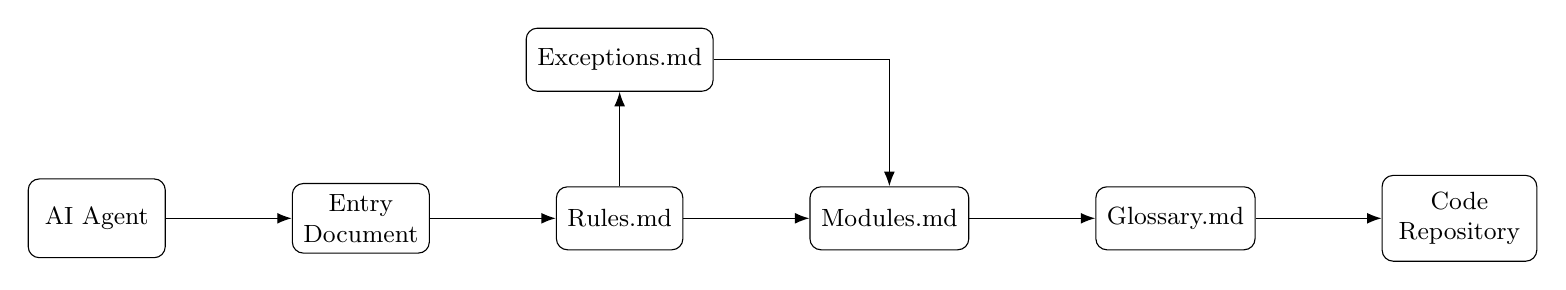
\begin{tikzpicture}[
  font=\small,
  node distance=12mm and 16mm,
  box/.style={draw, rounded corners, align=center, inner sep=6pt, minimum height=10mm},
  smallbox/.style={draw, rounded corners, align=center, inner sep=4pt, minimum height=8mm},
  arrow/.style={-Latex, line width=0.5pt}
]

% Nodes (left to right)
\node[box] (agent) {AI Agent};

\node[smallbox, right=of agent] (entry) {Entry\\Document};

\node[smallbox, right=of entry] (rules) {Rules.md};
\node[smallbox, above=of rules] (exceptions) {Exceptions.md};
\node[smallbox, right=of rules] (modules) {Modules.md};
\node[smallbox, right=of modules] (glossary) {Glossary.md};

\node[box, right=of glossary] (repo) {Code\\Repository};

% Traversal arrows (incremental navigation)
\draw[arrow] (agent) -- (entry);
\draw[arrow] (entry) -- (rules);

\draw[arrow] (rules) -- (modules);
\draw[arrow] (modules) -- (glossary);

\draw[arrow] (rules) -- (exceptions);
\draw[arrow] (exceptions.east) -| (modules.north);

% Final action toward code
\draw[arrow] (glossary) -- (repo);

\end{tikzpicture}}
\caption{Domain Navigation Layer (DNL) as a navigation interface: the agent incrementally traverses linked Markdown pages from an entry document to task-relevant rules, module knowledge, glossary terms, and exceptions before acting on the codebase.}
\label{fig:dnl-nav-layer}
\end{figure}


\section{Three-Level Architecture}
While the core concept of DNL is repository-agnostic, organizations typically operate multiple repositories, multiple products, and evolving conventions. To support scalability and systematic reuse, we extend DNL into a three-level hierarchy---Company, Product, and Project---where each level has a distinct scope, ownership boundary, and stability expectation. The hierarchy prevents duplication (by placing broadly applicable knowledge at higher levels) while keeping time-sensitive and implementation-specific knowledge close to the code (at the project level).

\begin{figure}[t]
\centering
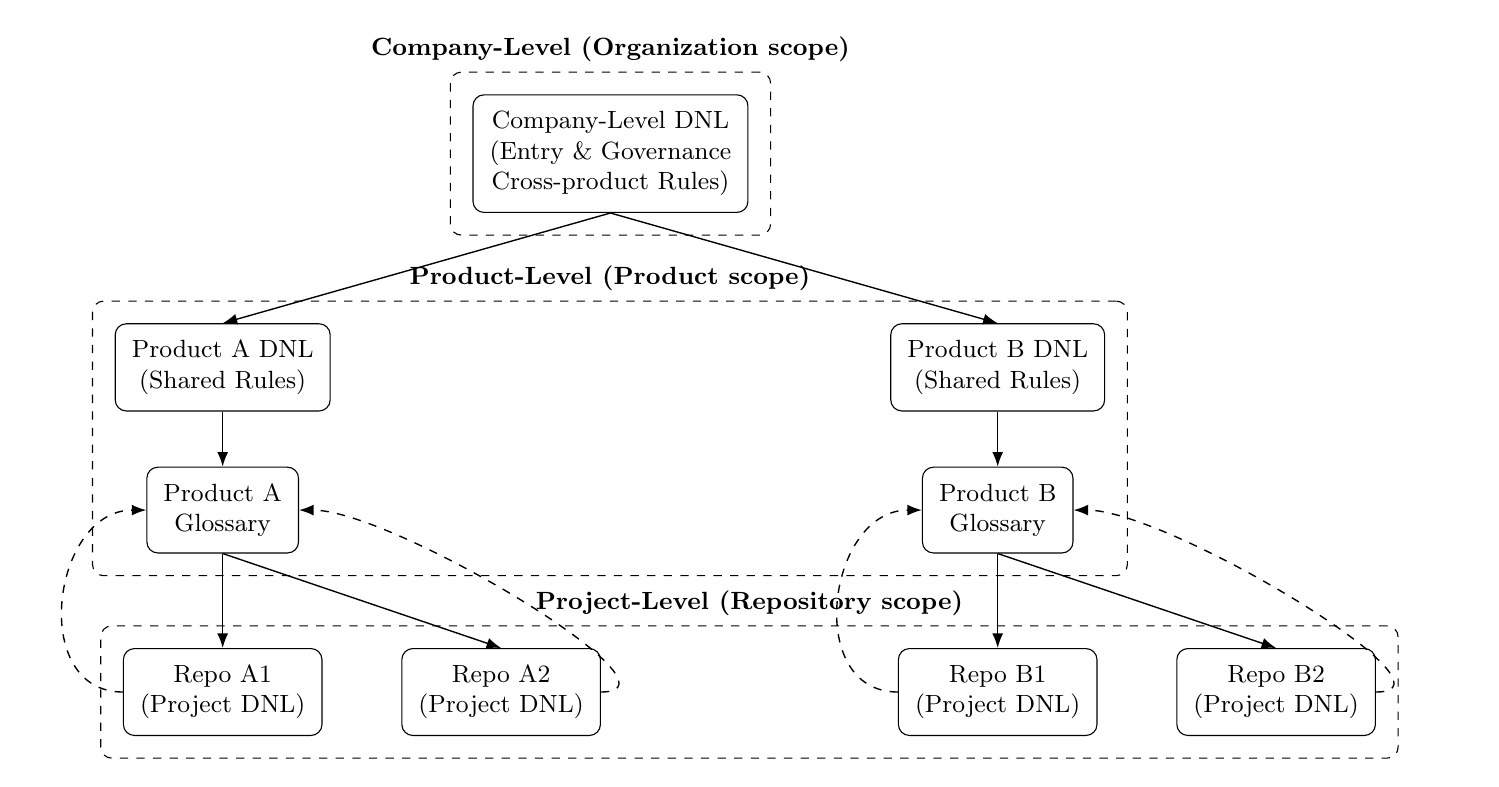
\begin{tikzpicture}[
  font=\small,
  >=Latex,
  box/.style={draw, rounded corners, align=center, inner sep=6pt},
  layer/.style={draw, dashed, rounded corners, inner sep=8pt},
  arrow/.style={-Latex, line width=0.5pt},
  cross/.style={-Latex, line width=0.5pt, dashed},
  node distance=10mm and 14mm
]

% Core nodes
\node[box] (company) {Company-Level DNL\\(Entry \& Governance\\Cross-product Rules)};

\node[box, below left=14mm and 18mm of company] (prodA) {Product A DNL\\(Shared Rules)};
\node[box, below right=14mm and 18mm of company] (prodB) {Product B DNL\\(Shared Rules)};

\node[box, below=7mm of prodA] (glossaryA) {Product A\\Glossary};
\node[box, below=7mm of prodB] (glossaryB) {Product B\\Glossary};

\node[box, below=12mm of glossaryA] (a1) {Repo A1\\(Project DNL)};
\node[box, right=10mm of a1] (a2) {Repo A2\\(Project DNL)};

\node[box, below=12mm of glossaryB] (b1) {Repo B1\\(Project DNL)};
\node[box, right=10mm of b1] (b2) {Repo B2\\(Project DNL)};

% Scope boundaries (dashed)
\node[layer, fit=(company), label={[align=center]above:\textbf{Company-Level (Organization scope)}}] {};
\node[layer, fit=(prodA)(prodB)(glossaryA)(glossaryB), label={[align=center]above:\textbf{Product-Level (Product scope)}}] {};
\node[layer, fit=(a1)(a2)(b1)(b2), label={[align=center]above:\textbf{Project-Level (Repository scope)}}] {};

% Inheritance arrows (downward)
\draw[arrow] (company.south) -- (prodA.north);
\draw[arrow] (company.south) -- (prodB.north);

\draw[arrow] (prodA.south) -- (glossaryA.north);
\draw[arrow] (prodB.south) -- (glossaryB.north);

\draw[arrow] (glossaryA.south) -- (a1.north);
\draw[arrow] (glossaryA.south) -- (a2.north);
\draw[arrow] (glossaryB.south) -- (b1.north);
\draw[arrow] (glossaryB.south) -- (b2.north);

% Cross-links (projects <-> product glossary)
\draw[cross] (a1.west) .. controls +(-12mm,0) and +(-12mm,0) .. (glossaryA.west);
\draw[cross] (a2.east) .. controls +(12mm,0) and +(12mm,0) .. (glossaryA.east);
\draw[cross] (b1.west) .. controls +(-12mm,0) and +(-12mm,0) .. (glossaryB.west);
\draw[cross] (b2.east) .. controls +(12mm,0) and +(12mm,0) .. (glossaryB.east);

\end{tikzpicture}
\caption{Three-level DNL architecture with scope boundaries, downward inheritance of conventions, and cross-links to product-level glossaries.}
\label{fig:dnl-three-level}
\end{figure}

\begin{figure}[t]
\centering
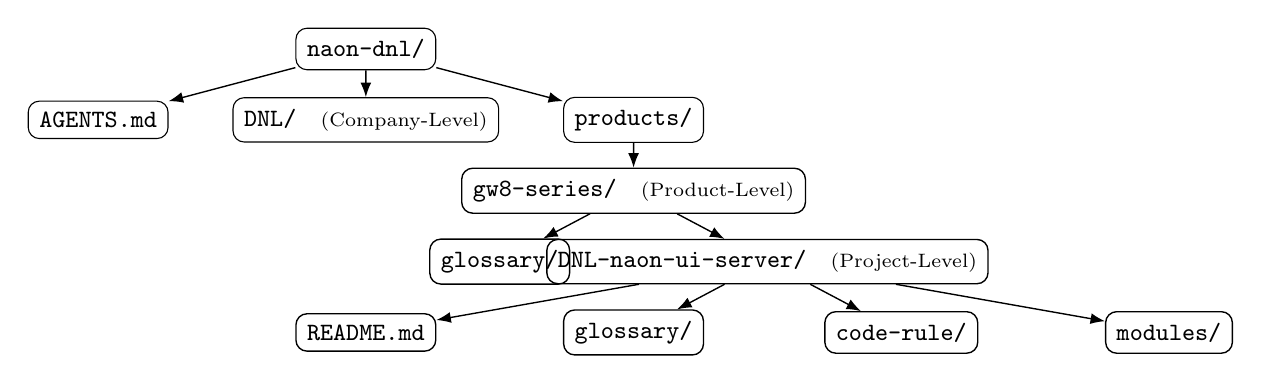
\begin{tikzpicture}[
  font=\small,
  level distance=9mm,
  sibling distance=34mm,
  edge from parent/.style={draw,-Latex,line width=0.5pt},
  every node/.style={draw, rounded corners, align=left, inner sep=4pt},
  grow=down
]

\node {\texttt{naon-dnl/}}
  child { node {\texttt{AGENTS.md}} }
  child { node {\texttt{DNL/} \hspace{2mm}\scriptsize (Company-Level)} }
  child { node {\texttt{products/}}
    child { node {\texttt{gw8-series/} \hspace{2mm}\scriptsize (Product-Level)}
      child { node {\texttt{glossary/}} }
      child { node {\texttt{DNL-naon-ui-server/} \hspace{2mm}\scriptsize (Project-Level)}
        child { node {\texttt{README.md}} }
        child { node {\texttt{glossary/}} }
        child { node {\texttt{code-rule/}} }
        child { node {\texttt{modules/}} }
      }
    }
  };

\end{tikzpicture}
\caption{Illustrative DNL directory structure spanning company-, product-, and project-level documentation.}
\label{fig:dnl-directory-structure}
\end{figure}

\subsection{Company-Level DNL}
The Company-Level DNL is the entry point and normative layer for an organization-wide DNL deployment. It specifies how agents (and humans) should use DNL, how documents are expected to be written and linked, and which process rules govern updates.
\paragraph{Usage philosophy.} This level defines the organization’s assumptions about ``what must be true'' for an agent to act safely, such as the expectation that decisions cite DNL pages, and that domain rules take precedence over ad hoc prompt instructions when conflicts arise.
\paragraph{Process rules.} It defines governance mechanisms (e.g., ownership, review requirements, deprecation policy, and versioning conventions) to keep DNL auditable and to reduce drift.
\paragraph{Cross-product conventions.} It records conventions that span products, such as security requirements, privacy classifications, reliability targets (SLO/SLA terminology), incident practices, naming conventions, and standard integration patterns. Because these conventions apply broadly, placing them at the company level eliminates repeated restatement in each product.

\subsection{Product-Level DNL}
The Product-Level DNL captures knowledge shared across multiple repositories that jointly implement a single product or platform. This level is the primary locus for cross-repository consistency and integration correctness.
\paragraph{Cross-repository shared knowledge.} It documents the product architecture, service boundaries, shared data models, and inter-service contracts that cannot be understood from any single repository.
\paragraph{Infrastructure and integration rules.} It specifies operational and integration constraints such as deployment environment assumptions, authentication/authorization mechanisms, messaging and API standards, backward compatibility policies, and migration procedures.
\paragraph{Shared glossary.} It provides a product-scoped vocabulary for domain entities and metrics, reducing ambiguity across teams and enabling agents to map user intent to the correct artifacts.

\subsection{Project-Level DNL}
The Project-Level DNL is scoped to a single Git repository and is maintained closest to code. It prioritizes concreteness and task-execution guidance.
\paragraph{Code rules.} It records repository-specific coding standards, testing requirements, build/deploy commands, error-handling conventions, and non-obvious invariants that are easy to violate.
\paragraph{Module documentation.} It describes modules/packages, their responsibilities, public interfaces, and local design rationale, with links back to product-level concepts for shared abstractions.
\paragraph{Local glossary and patterns.} It defines repo-local terms (e.g., abbreviations, table names, internal event names) and catalogs common patterns (e.g., how to add a new endpoint, how to introduce a feature flag, how to extend a state machine) in a form that agents can follow.

\paragraph{Scalability and reuse.}
The three-level hierarchy improves scalability by separating stable, high-leverage knowledge (company and product) from volatile implementation detail (project), allowing updates to propagate without repetitive edits. It also improves knowledge reuse by making shared constraints and vocabulary linkable dependencies: project pages can reference product/company pages instead of duplicating them, enabling agents to build task-specific context through a consistent, hierarchical traversal path.

\section{Case Study}
This section reports observations from applying DNL to \texttt{naon-ui-server}, a real Git repository developed within a larger enterprise product. The goal of the case study is not to claim general performance gains, but to analyze how a structured navigation layer changes the interaction between an AI agent and domain knowledge during realistic engineering tasks.

\subsection{Context of the project}
\texttt{naon-ui-server} implements server-side UI logic and related application services for an enterprise product. The repository is organized into domain-facing modules (e.g., \texttt{board}, \texttt{organization}, \texttt{mail}) and includes recurring architectural patterns (e.g., shared request/response shapes, authorization checks, and module-scoped boundaries). In practice, correctness depends on conventions that are only partially visible in code: internal terminology, cross-module invariants, and organization-specific rules for how modules are introduced and extended.

\subsection{Problem before DNL}
Prior to introducing DNL, AI-assisted development exhibited inconsistent behavior across similar prompts. When asked to implement or modify features, the agent often inferred plausible but non-conforming conventions (e.g., inventing endpoint shapes, misnaming domain entities, or applying an authorization pattern used in a different module). These errors were not primarily syntactic; they reflected missing domain conventions and ambiguity in terms that appear natural-language-equivalent but have repository-specific meanings. Moreover, attempts to mitigate the issue by providing more files in the prompt were limited by token budgets and by context fragmentation: each task required a different subset of documents, and repeated manual curation was not reproducible.

\subsection{DNL-based navigation process}
We introduced DNL documents for \texttt{naon-ui-server} and linked them in a consistent traversal order from rules to modules to glossary. The intent was to make the agent's knowledge acquisition explicit and repeatable.

\paragraph{Step-by-step example.}
Consider the task: \emph{add a new ``announcement'' capability under the \texttt{board} module, including an API to create and list announcements}. Under DNL, the agent is instructed to follow a fixed navigation procedure before proposing code changes:
\begin{enumerate}
  \item \textbf{Read code rules.} Start from the project entry page and read \emph{Code Rules} (repository-specific constraints such as routing conventions, validation patterns, error handling, and test expectations).
  \item \textbf{Identify the module boundary.} Follow links to \emph{Modules} and then to \texttt{board} to learn the module’s responsibility, existing endpoints, and any local invariants.
  \item \textbf{Resolve terminology.} Follow links from the \texttt{board} page to the \emph{Glossary} to disambiguate terms such as ``post'', ``notice/announcement'', ``organization scope'', and identifiers used in payloads.
  \item \textbf{Check cross-module patterns.} If the \texttt{board} page links to shared patterns (e.g., authorization model or pagination conventions), read those pages before writing an implementation plan.
  \item \textbf{Act with citations.} Produce an implementation plan that cites the consulted DNL pages (rules, module doc, glossary), then locate the corresponding code entry points and implement.
\end{enumerate}
This procedure makes the agent’s context expansion deterministic: documents enter the context window through explicit links, rather than through ad hoc prompt stuffing.

\begin{figure}[t]
\centering
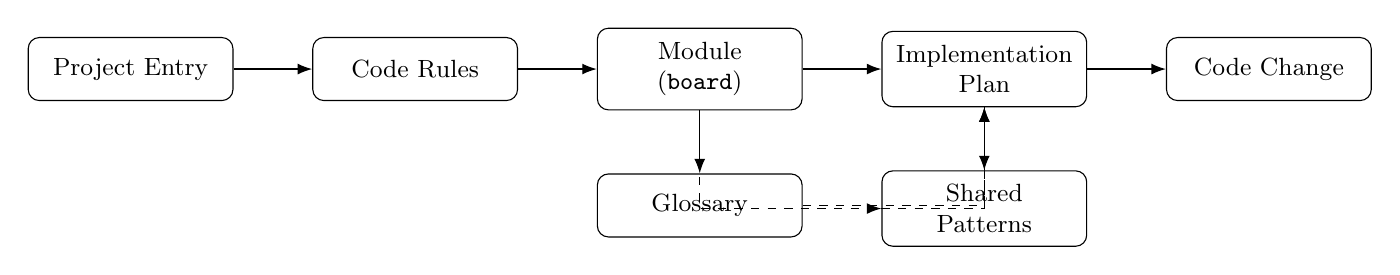
\begin{tikzpicture}[
  font=\small,
  node distance=8mm and 10mm,
  flowstep/.style={draw, rounded corners, align=center, inner sep=5pt, minimum height=8mm, minimum width=26mm},
  arrow/.style={-Latex, line width=0.5pt},
  back/.style={-Latex, line width=0.5pt, dashed}
]

% Main linear flow
\node[flowstep] (entry) {Project Entry};
\node[flowstep, right=of entry] (rules) {Code Rules};
\node[flowstep, right=of rules] (module) {Module\\(\texttt{board})};
\node[flowstep, right=of module] (plan) {Implementation\\Plan};
\node[flowstep, right=of plan] (change) {Code Change};

\draw[arrow] (entry) -- (rules);
\draw[arrow] (rules) -- (module);
\draw[arrow] (module) -- (plan);
\draw[arrow] (plan) -- (change);

% Branch: Glossary (may branch and return)
\node[flowstep, below=of module] (glossary) {Glossary};
\draw[arrow] (module.south) -- (glossary.north);
\draw[back] (glossary.east) -| (plan.south);

% Branch: Shared Patterns (may branch and return)
\node[flowstep, below=of plan] (patterns) {Shared\\Patterns};
\draw[arrow] (plan.south) -- (patterns.north);
\draw[back] (patterns.west) -| (plan.south);

% Optional: module may trigger pattern lookup
\draw[back] (module.south) |- (patterns.west);

\end{tikzpicture}
\caption{DNL-based navigation process observed in the \texttt{naon-ui-server} case study. Branches (glossary/patterns) represent on-demand context expansion with return to planning.}
\label{fig:naon-dnl-flow}
\end{figure}

\begin{figure}[t]
\centering
\fbox{%
\parbox{0.96\linewidth}{%
\small
\textbf{Navigation Trace Example (\texttt{naon-ui-server})}\\
\textbf{Task:} Add an announcement capability under the \texttt{board} module.\\[2mm]
\textbf{Navigation trace:}
\begin{enumerate}
  \item[\texttt{[1]}] \textbf{Project Entry} $\rightarrow$ locate module index and operational boundaries.
  \item[\texttt{[2]}] \textbf{Code Rules} $\rightarrow$ routing, validation, error handling, tests.
  \item[\texttt{[3]}] \textbf{Modules/\texttt{board}} $\rightarrow$ existing endpoints, responsibilities, invariants.
  \item[\texttt{[4]}] \textbf{Glossary} $\rightarrow$ disambiguate ``announcement'', identifiers, scope terms.
  \item[\texttt{[5]}] \textbf{Shared Patterns} $\rightarrow$ pagination, authorization, response envelope conventions.
\end{enumerate}
\vspace{1mm}
\textbf{Extracted constraints:}
\begin{itemize}
  \item The new capability must remain within the \texttt{board} module boundary and reuse its routing structure.
  \item Request/response schemas must follow repository-standard validation and error conventions.
  \item Terms used in API payloads must match glossary-defined meanings and identifiers.
  \item Authorization checks must follow the shared pattern referenced for module endpoints.
  \item List endpoints must conform to the shared pagination/filtering convention (if applicable).
\end{itemize}
}%
}
\caption{Example of an explicit navigation trace and extracted constraints prior to implementation.}
\label{fig:naon-navigation-trace}
\end{figure}

\subsection{Observed improvements}
\noindent\textbf{Before vs. After (comparative summary).}
\begin{center}
\begin{tabular}{p{0.26\linewidth}p{0.34\linewidth}p{0.34\linewidth}}
\hline
\textbf{Dimension} & \textbf{Before DNL} & \textbf{After DNL} \\
\hline
Context acquisition method & Ad hoc prompt curation and partial retrieval of scattered artifacts. & Link-guided traversal (rules $\rightarrow$ modules $\rightarrow$ glossary) with explicit prerequisites. \\
Consistency across sessions & Sensitive to prompt phrasing and the specific file bundle provided. & More stable due to repeated navigation paths and fixed reading-order rules. \\
Hallucination risk & Elevated when conventions/terms are missing from the immediate context. & Lowered by requiring definition lookup via linked glossary and pattern pages. \\
Token usage pattern & ``Front-loaded'' prompts with broad file inclusion; frequent truncation. & Incremental expansion; only task-relevant pages are loaded on demand. \\
Traceability of decisions & Implicit; difficult to reconstruct which assumptions drove a change. & Explicit; decisions can cite the consulted DNL pages and link paths. \\
\hline
\end{tabular}
\end{center}

We observed four qualitative changes after adopting DNL.
\paragraph{Consistency.} For repeated tasks of the same class (e.g., adding a route under an existing module), the agent produced plans that adhered to the same conventions across sessions, because the same ``rules $\rightarrow$ modules $\rightarrow$ glossary'' path was followed.
\paragraph{Reduced hallucination.} The frequency of invented entities and mismatched terminology decreased, especially for nouns with overloaded meanings (e.g., module-specific names that differ from generic UI/server terminology). The agent more often asked for, or retrieved via links, the missing definition rather than guessing.
\paragraph{Token efficiency.} Compared to providing large code excerpts and multiple READMEs by default, DNL enabled smaller initial prompts and incremental expansion: only the minimal set of pages required for the decision were loaded, while the remainder stayed available via navigation.
\paragraph{Analytical traceability.} Because the navigation path and cited pages were explicit, it became easier to audit why an implementation plan adopted a particular convention, and to correct the knowledge base when conventions changed (by updating the relevant DNL page rather than re-prompting with different file bundles).

\section{Related Work}
DNL is closely related to several lines of work on providing external knowledge and structure to large language models, but it differs in its emphasis on a \emph{navigation layer} that constrains how context is expanded under token budgets.

\paragraph{Retrieval-Augmented Generation (RAG).}
RAG-based systems address context limitations by retrieving potentially relevant passages from an indexed corpus and injecting them into the prompt. In software engineering settings, retrieval can be effective for locating code or documentation fragments, but it can also be sensitive to query formulation, embedding drift, and ranking errors. DNL is complementary: instead of treating retrieval as the primary mechanism for grounding, DNL encodes stable, human-curated traversal paths (prerequisites, exceptions, and scope boundaries) that can guide retrieval and reduce ambiguity in what should be read next.

\paragraph{Agentic coding workflows.}
Recent agentic approaches decompose development tasks into iterative planning, tool use, and verification cycles. While such workflows improve autonomy, they often rely on ad hoc context selection and repeated summarization, which can amplify inconsistency across runs. DNL targets this bottleneck by making context acquisition a first-class, repeatable procedure: the agent follows links in a prescribed order (e.g., rules $\rightarrow$ modules $\rightarrow$ glossary) before producing plans or edits.

\paragraph{Knowledge graphs and structured representations.}
Knowledge graph approaches represent entities and relations explicitly to support reasoning and retrieval. DNL shares the motivation of making relationships explicit, but adopts a lightweight representation: linked Markdown pages and link semantics serve as a pragmatic graph that remains easy to author and review. Unlike schema-heavy graph constructions, DNL focuses on operational guidance and reading order rather than on formal inference.

\paragraph{Software documentation methodologies.}
Documentation practices such as architecture decision records, design docs, and modular READMEs aim to preserve rationale and reduce onboarding cost. DNL aligns with these goals but reframes documentation as an interface for AI context management: documents are written to be traversed incrementally, with explicit prerequisites and exception handling, so that an agent can remain within a bounded context window while still accessing the full corpus through navigation.

\section{Limitations and Future Work}
DNL shifts a portion of the ``alignment'' burden from interactive prompting to a maintained knowledge layer. This shift has a clear cost: documentation must be written, curated, and kept consistent with evolving code and organizational practices. In environments where ownership is unclear or change velocity is high, the maintenance overhead can become non-trivial, and neglected pages may degrade rather than improve agent performance.

A second limitation concerns link integrity and knowledge freshness. DNL relies on stable traversal paths: broken links, renamed concepts, or partially updated pages can lead an agent to incomplete or outdated constraints. More subtly, even when links resolve, content can become stale as APIs, architectural patterns, or policies change. This creates a failure mode in which an agent behaves consistently yet incorrectly, because it is consistently guided by obsolete rules. Mitigating this requires explicit deprecation mechanisms, timestamps or applicability conditions, and regular review cycles.

DNL also presupposes organizational discipline. Effective use requires shared conventions for page structure, naming, and the semantics of links (e.g., prerequisite vs. related vs. exception). Without this discipline, the document graph can become inconsistent, and agents may not follow comparable paths across tasks. Moreover, governance questions arise: who is authorized to change normative pages, how disagreements are resolved, and how exceptions are represented without fragmenting the knowledge base.

Finally, there is a risk of over-formalization. Attempting to encode every nuance as explicit rules can produce documents that are difficult to read, discourage contribution, or prematurely freeze practices that should remain flexible. DNL should therefore be treated as an interface for decision-relevant constraints and vocabulary, not as a complete specification of a socio-technical system; choosing what \emph{not} to formalize is part of the design.

Future work centers on reducing maintenance burden and improving reliability via automation. Promising directions include link validation tools (e.g., continuous checks for broken or circular dependencies), DNL linting bots that enforce formatting and reading-order conventions, and integration with indexing systems (including MCP-like tool interfaces) to support hybrid retrieval and navigation. Another direction is automated navigation-trace logging, whereby an agent records the sequence of consulted DNL pages and the extracted constraints, enabling post hoc audits and facilitating targeted updates to the knowledge layer when failures occur.

\bibliographystyle{plain}
\bibliography{refs}

\end{document}
